\chapter{Accessibility}
\label{ch:accessibility}
% ##################################################################################################################

\hfill \textbf{Author:} Dominik Ziemke

\begin{center} 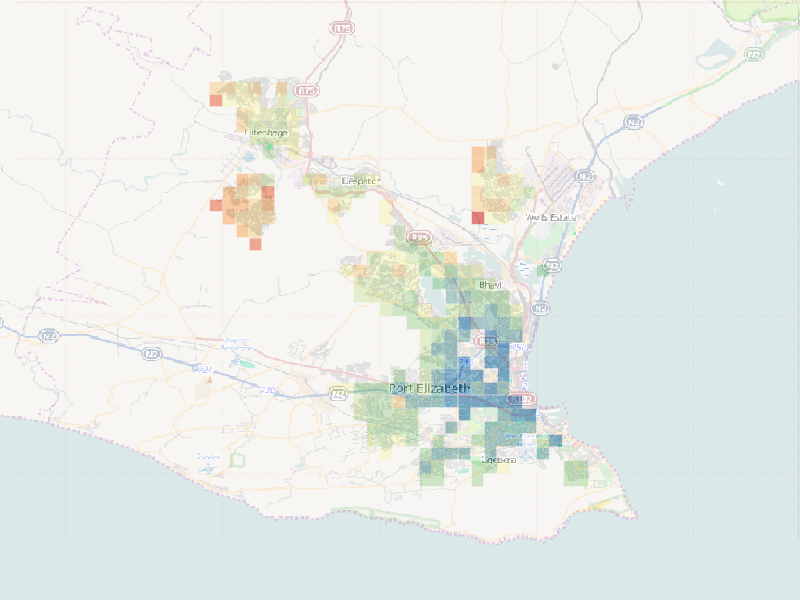
\includegraphics[width=0.5\textwidth, angle=0]{extending/figures/accessibility/w_freeSpeed_snapshot.png} \end{center}

\createStandardInformation{accessibility}{\lstinline{RunAccessibilityExample} class}{accessibility}{\citet{NicolaiNagel2012HiResAccessibilityMethodInBook}}

% ##################################################################################################################

\mnote{wider context}
In transport science and planning, the term accessibility can refer to at least three different concepts. 
First, accessibility may be used to describe how well a certain component of the transport infrastructure 
is useable by citizens, in particular by handicapped people \citep{Faura2012AccessibilityEvaluationTrafficSimulation}. 
In this sense, \textit{accessibility guidelines} tell engineers and planners how to design transport 
infrastructure elements, such as public transport facilities, to make them accessible, \ie useable 
for all citizens. Second, accessibility may be used to describe how easy and convenient the approach 
towards a given land-use facility is. There are, for instance, studies \citep{Fujiyama2004AccessibleDesignPTFacilities} 
that seek to improve the accessibility of shopping centers by redesigning the access roads and their 
connection to major roads. Finally, the term accessibility can be used in a more global fashion to 
describe the availability and spatial distribution of activity facilities within a given area, \eg a 
metropolitan region, and the ease with which these facilities can be reached from other locations of 
the region. The accessibility extension of \gls{matsim} is concerned with this notion of accessibility. 
Its discussion in this chapter draws on \citet{NicolaiNagel2012HiResAccessibilityMethodInBook}.

% ##################################################################################################################
\section{Introduction}
The improvement of accessibility is often stated as a central goal of proposed transport or infrastructure 
schemes \citep{GeursEtAl2012AccessibilityTransportIntroduction}. Not in all contexts, in which the term 
accessibility is discussed, however, it used as a precisely-defined, quantitative measure. While 
\citet{Batty2009AccessibilityUnifiedTheory} traces the origins of the concept of accessibility back to 
location theory and regional economic planning of the 1920s when transport planning began in North America
\citep{GeursEtAl2012AccessibilityTransportIntroduction}, 
Hansen, with his widely-cited paper \citep{Hansen1959HowAccessibilityShapesLandUse}, is generally credited 
with the first real definition of accessibility. He defines accessibility 
as \textit{the potential of opportunities for interaction} 
%also said so e.g. in Gulhan p.130
A bit more illustrative, \citet{MorrisEtAl1978AccessibilityIndicators} define accessibility as 'the ease with 
which activities may be reached from a given location using a particular transportation system'.
%\citet{DalviMartin1976MeasurementAccessibility} define accessibility as 'the ease with which any 
%land-use activity can be reached from a location using a particular transport system'. 
% I (dz) I think the above citation is wrong; read this somewhere, but dont know anymore where it was
The concept of accessibility is seen as a potential alternative or supplement for the assessment 
of transport systems as it is a more comprehensive and inclusive way to evaluate how, where and why 
people move as it takes the well-known dependencies between transport and land use into account.
\citet{Hansen1959HowAccessibilityShapesLandUse} appears to be the first to have developed a procedure for 
the quantitative consideration of accessibility, which is discussed in more detail in section 
\ref{sec:potential}.

%MorrisEtAl1978AccessibilityIndicators, p.92
%accessibility indicators provide possibly the most useful and appropriate means of summarising a great deal of 
%information on the location of households in relation to the distribution of urban activities and the transport 
%system that connects them (Wachs 1978)

%CurtisEtAl2013AccessbilityPolicyInnovation, p.471, definition:
%Accessibility here is defined as the ease or convenience of reaching a destination and is measured by the number 
%of people with access to certain land-use activities or facilities (opportunities) as well as to the transport 
%network itself. This is different to the way some conceive accessibility where it has been used in relation to 
%the mobility needs of elderly or disabled populations (universal accessibility).

%from ERAfrica proposal
%The term “accessibility” has recently gained attention as a potential alternative and state-of-the-art metric as 
%it is a more comprehensive and inclusive way to evaluate how, where and why people move. Accessibility focuses 
%less on the quality and quantity of travel, and more on the needs of households and individuals. Axhausen et al (2011) 
%highlight that accessibility requires knowledge of the activity opportunities for the population, the population 
%characteristics itself, and the generalized cost of travel between activities. With generalized cost we mean the 
%sum of monetary and non-monetary costs. Definitions by Bocarejo and Oviedo (2012), Knowles (2009) and Litman 
%(2010) all emphasize the ease with which individuals have access to goods, services, employment, education, etc. 
%Litman (2010) refers to these activity types, that individuals wish to participate in, collectively as opportunities. 
%Other definitions focus on the mere ability to access opportunities, as opposed to the ease of access (Fan and 
%Huang, 2011; Gutirrez, 2009). In contrast to access, which measures the cost of reaching one particular location 
%and opportunity, accessibility measures the set of all potentially reachable opportunities and is in this way, a 
%measure of total quality of a location as a starting place from the point of view of a traveller. Adopting the 
%point of view of a supplier accessibility measures the potential in terms of visitors or customers to that location 
%as a destination.

%BuettnerEtAl2010Erreichbarkeitsatlas, p.43
%Erreichbarkeit ist **keine** eindeutig definierte Größe. Stattdessen wurden über die letzten Jahrzehnte 
%verschiedene Ansatze zur Quantifizierung des schwer fassbaren Erreichbarkeitsbegriffs entwickelt. Eine 
%weitreichende Einigkeit herrscht in der Wissenschaft allerdings darüber, dass sich Erreichbarkeitsindikatoren 
%durch die Eigenschaft auszeichnen, Merkmale der Siedlungsstruktur einerseits und des Verkehrsangebots 
%andererseits zusammenzuführen


\mnote{typology}
%Depending on the concrete definition of quantitative accessibility measures, the explanatory power of the 
%result varies widely. As pointed out by \citet{GeursRitsema2001AccessibilityMeasures} (\citep[see also][]{Geurs2004AccessibilityReview}), quantitative indicators can rely on the following approaches:
In their widely-cited review, \citet{Geurs2004AccessibilityReview} identify four components of accessibility 
from different existing definitions and applied measures of accessibility:

\begin{enumerate}\styleEnumerate
	\item The \textbf{land-use} component reflects
	the number and spatial distribution of opportunities.
	
	\item The \textbf{transport} component describes the effort
	to travel from a given origin to a given destination.
	
	\item The \textbf{temporal} component considers the availability of activities at
	different times-of-day, \eg in the morning peak hours.
	
	\item The \textbf{individual} component addresses the different needs and
	opportunities of different socio-economic groups, \eg different income groups.
\end{enumerate}

%\begin{enumerate}
%\item An \textbf{activity-based} or \textbf{land-use-based} approach focuses on
%the distribution of possible activity locations (land use). One can, for instance,
%base calculations on the number and spatial distribution of activity opportunities
%like shopping locations or workplaces within a certain distance.
%%
%\item An \textbf{in\-fra\-struc\-ture-based} or \textbf{transport-based} approach takes into account the effort 
%to travel from a given origin to a given destination and 
%can be based on performance characteristics of the transport system, e.g. the
%average speed by mode at certain locations. If one considers, for instance, the
%number of shopping locations or workplaces under a defined travel time threshold,
%the activity-based and the infrastructure-based approaches can be combined.
%%
%\item A \textbf{temporal} component, which considers the availability of activities at
%different times-of-day, may be added.
%%
%\item An \textbf{individual} approach to accessibility computations can be
%obtained by addressing different needs and opportunities of different socio-economic groups, \eg different income groups.
%%
%\item A \textbf{utility-based} measurement of accessibility reflects the
%(economic) benefits, as the maximum expected utility, that someone gains
%from access to spatially distributed opportunities
%\citep{GeursRitsema2001AccessibilityMeasures,deJongEtAl2007LogsumTRA}. The
%typical example is the logsum term, which is discussed further below.
%\end{enumerate}

In this review, \citet{Geurs2004AccessibilityReview} list and summarize typical approaches applying the concept 
of accessibility, which have their focus on different of the aforementioned components of accessibility:

\begin{enumerate}\styleEnumerate
	\item \textbf{Infrastructure-based} measures focus on the (observed or simulated) performance or service level 
	of transport infrastructure, \eg represented as average travel speed. These kind of measures are typically used 
	in transport planning.
	
	\item \textbf{Location-based} measures describe the level of accessibility to spatially distributed activities, such as 
	the number of jobs within 30\,minutes travel time from origin locations. These kind of measures are typically used 
	in urban planning and geographical studies.
	
	%CurtisEtAl2013AccessbilityPolicyInnovation, p.456
	%Activity- or destination-based accessibility modelling has expanded rapidly with the coalescing of advanced GIS
	
	\item \textbf{Person-based} measures analyze accessibility at the individual level, such as the activities in which an 
	individual can participate at a given time. These kind of measures are founded in the space–time geography 
	of \citet{Haegerstrand1970}.
	
	\item \textbf{Utility-based} measures analyze the economic benefits that people derive from access to spatially 
	distributed activities. These kind of measure have their origin in economic studies.
\end{enumerate}

\citet{Geurs2004AccessibilityReview} intersect these typical approaches with the four components of accessibility identified 
above, which leads to a matrix. This matrix illustrates how each of the four aforementioned components of accessibility is 
typically represented in the four different accessibility measures, where each measure is typically concerned with certain weaknesses 
in terms of those accessibility components, which are not the particular focus of the given kind of measure. Accordingly, \citet{Geurs2004AccessibilityReview} assert that it would be desirable if an accessibility measure included 
all four aforementioned components of accessibility. The accessibility extension of \gls{matsim}, as will be described in 
the following, can be seen as an approach to achieve this goal.

\mnote{latest research}
In other recent strands of research, as identified by \citet{GeursEtAl2012AccessibilityTransportIntroduction},
the concept of accessibility is also applied to the analysis of social exclusion (\eg by examining the benefit 
disadvantaged populations in terms of employment accessibility before and after the implementation of a 
transport scheme), the economic valuation of accessibility effects (\eg in cost-benefit analyses and studies 
assessing the impact of changes in public transport accessibility on house prices), and the analysis of behavior 
with accessibility measures (\eg walking behavior dependent on different qualities of residential neighborhood 
accessibility). It has furthermore been used to explore questions of oil vulnerability, climate change, and 
other emergent concerns \citep{CurtisEtAl2013AccessbilityPolicyInnovation}.

%CurtisEtAl2013AccessbilityPolicyInnovation, p.455f
%New forms of transport analysis are emerging that can be used, in addition to the traditional transport models, 
%to expand knowledge and enable a fuller range of policy issues to be examined. Advances in the rise of geographic 
%information systems (GIS) has allowed for new methods to explore questions of equity and access (Halden, 2002), oil 
%vulnerability (Dodson and Sipe, 2007), climate change (Hickman et al., 2010) and other emergent concerns. Activity- or 
%destination-based ac- cessibility modelling has expanded rapidly with the coalescing of advanced GIS, comprehensive 
%spatial datasets, exemplar projects and skills development in the planning and transport professions

%MorrisEtAl1978AccessibilityIndicators, p.92
%The two principal bases of classification are the behavioural dimension mentioned earlier, and a dis- tinction between 
%“relative accessibility” and “ integral accessibility” developed by Ingram (1971). Relative accessibility describes the 
%relation or degree of connection between any two points, whereas integral accessibility describes the relation or-degree 
%of interconnection be- tween a given point and all others within a spatial set of pointst (see Fig. 2.)

\section{The Measure of Potential Accessibility}
\label{sec:potential}
\mnote{measures in practice}
Today, methods to assess the quality of accessibility are often used in superordinate planning procedures like 
regional transport planning, where a central goal is to provide 
citizens with a certain quality of access to various services. For instance, the approach used by Germany's agency 
responsible for regional planning calculates travel times to major service facilities like airports or hospitals \citep{BBSR20xxErreichbarkeitsmodell}. The results, typically visualized by multi-colored maps, give useful insights 
into the supply of the population with certain services and can therefore assist the planning of the (transport) 
infrastructure in light of the goal to improve this supply.
% transport component
% As such, this definition of an accessibility measure has its focus on the \textbf{trasnport component} of accessibility 
% as introduced above.
Since in this approach travel times to the \textit{next} airport, to the \textit{next} hospital, and to the \textit{next} 
autobahn access are calculated, the implicit assumption is made that citizens' needs are fulfilled by one (i.e the \textit{next} 
or closest in terms of travel times) facility of a given type.

%BuettnerWulfhorstEtAl2013Vulnerability, p.13
%given number of jobs accessible by a given mode of transport (here: public transport) within a given amount of time (here: 
%60min) displayed in a colored my by municiplaity, i.e. on a zone-based level; data source: Erreichbarkeitsatlas
%BuettnerWulfhorstEtAl2013Vulnerability, p.14
%basically the same for Lyon: Isochrone accessibility to jobs is measured for public transport commuters, in the morning 
%peak period. Travel time is computed using a “shortest path algorithm”

\mnote{land-use component}
An accessibility measure becomes insightful, however, if not only the impedance to reach \textit{the nearest} facility 
serving a particular need is taken into account, but instead a \textit{set of multiple reachable} facilities serving the same 
need is considered. This is due to the fact that different facilities of the same type may offer a given service in 
different qualities. Also, services may become more beneficent when combined with complementary services provided by 
another facilities of the same type. For instance, a person wishing to make a holiday trip by airplane will likely 
take into account several airports in their vicinity when planning a journey instead of just looking at the flights 
offered from the nearest airport. Therefore, the accessibility to airports should be made dependent on the impedance 
to reach all of these airports instead of just the impedance to reach the nearest one. Facilities offering medical 
services may serve as another example. Only taking into account the nearest hospital may be sufficient when looking 
at simple services like first aid, which can be assumed to be available at almost \textit{any} hospital. In other cases, 
however, the supply with medical services will be better represented by considering several hospitals in the vicinity 
because they are likely to offer different kinds of medical treatment that complement each other. 
% land-use componenent
The consideration of the set of multiple facilities, which are potentially useful from the perspective of a citizen residing
at a given location, corresponds to respecting the \textbf{land-use component} of accessibility as defined above.

\mnote{potential accessibility}
An approach that pursues the idea of taking into account the whole scope of potential activity facilities is the one 
developed in Hansen's early study \citep{Hansen1959HowAccessibilityShapesLandUse}, where an accessibility 
measure referred to as \textit{potential accessibility} is defined. Such measures of potential accessibility are 
specified as the (weighted) sum over the 
accessibilities of several facilities of a given activity type (\eg shopping, leisure etc.) and are of the mathematical form
%The (quantitative) accessibility measure in the MATSim accessibility extension is of the mathematical form
\begin{equation}
	A_i = g\Big( \sum_j a_j \, f(c_{ij}) \Big) \ ,
	\label{eq:accessibility:basic}
\end{equation}
where the sum goes over all possible destinations (opportunities) $j$, $a_j$ is an indicator of the attractiveness of 
the opportunity, $c_{ij}$ is the generalized cost of travel to get from $i$ to $j$, $f(c)$ is an impedance function 
that typically decreases with increasing distance, and $g(.)$ is an arbitrary, but typically monotonically increasing, 
function. 
%That is, the accessibility at $i$ is computed from a weighted sum over all possible destinations, where the weight is 
%the product of the destination's attractiveness and the ease to get there.
The weight is the product of the destination's attractiveness and the ease to get there. As can be seen by its 
functional form, this type of accessibility measure is related to gravity models used in trip generation models, which 
is why this measure is sometimes also referred to as a ``gravity type'' accessibility indicator 
\citep{MorrisEtAl1978AccessibilityIndicators}. The (quantitative) accessibility measure used in the \gls{matsim} 
accessibility extension is of this mathematical form and may thus be seen as a \textit{potential accessibility} measure.

%MorrisEtAl1978AccessibilityIndicators, p.94
%the “gravity type” indicators, as introduced by Hansen (1959), lend themselves to a variety of functional forms of 
%impedance (power, exponential, Gaussian, etc.)

%BuettnerEtAl2010Erreichbarkeitsatlas, p.44
%Die methodische Grundidee der ortsbezogenen Erreichbarkeitsindikatoren liegt darin, dass ein Ausgangsstandort
%mit allen gegebenen Zielstandorten bzw. Teilraumen innerhalb des definierten Untersuchungsgebiets in Beziehung 
%gesetzt wird. Jedem Ziel- standort ist ein Potenzial zugeordnet. Die Summe dieser Potenziale ist die Erreichbarkeit 
%des Ausgangsstandorts. Das Potenzial eines Zielstandorts wird dabei in der Regel durch die strukturelle Große dieses 
%Standorts definiert (z.B. Einwohnerzahl, Verkaufsflache). Allerdings wird in Abhängigkeit des Raumwiderstands 
%(Reisezeit, Kosten etc.), der für die Reise vom Ausgangs- zum Zielstandort überwunden werden muss, eine Abwertung 
%des Potenzials vorgenommen.

\mnote{ingoing vs. outgoing accessibility}
At this point, it may be important to note that the above-defined measure quantifies how good the accessibility \textit{to} 
certain services from a given location $i$ as the origin is. This kind of accessibility may therefore be referred to 
as ``outgoing'' accessibility, while a measure of ``ingoing'' accessibility would quantify how well a given destination 
location $j$ is accessible \textit{from} other locations. \citet{NicolaiNagel2012HiResAccessibilityMethodInBook} 
discuss under which circumstances both measures are interchangeable.

\section{Accessibility Computation integrated with Transport Simulation}
\label{sec:integrated}
\mnote{transport component}
\mnote{uncongested vs. congested network}
As mentioned above, accessibility computations are oftentimes based on travel times 
\citep{BBSR20xxErreichbarkeitsmodell, BuettnerEtAl2010Erreichbarkeitsatlas}
%###################################################################
%more citations if I remember who stated this fact as well
, which serve as an impedance measure. The way of calculating these travel times can, however, vary significantly. 
The most simple approach to calculate a travel time between two locations is measuring the Euclidean distance 
(beeline distance) between these two locations and then, by means of some kind of average speed, approximate the 
travel time between these two locations. According to \citet{Geurs2004AccessibilityReview}, this is the usual 
approach in location-, person-, and utility-based accessibility approaches, i.e. those approaches where the focus 
is not explicitly on the consideration of the transport system.

%CurtisEtAl2013AccessibilityPolicyInnovation, p.458
%This led to the development of an impediment measure based on properties most closely related to users’ experience: 
%that is, travel time, journey transfer and frequency of service, rather than geographical distance.

%BuettnerEtAl2010Erreichbarkeitsatlas, p.49
%Erreichbarkeit berechnet sich gemaß des dargestellten Konzepts einerseits aus den Potenzialen, der im Untersuchungsgebiet 
%liegenden Standorte (dies konnen z.B. Verkehrszellen sein) sowie andererseits aus den Widerständen der Raumuberwindung, 
%welcher der Einfachheit halber meist durch die Reisezeiten abgebildet werden

In order to strengthen the \textbf{transport component} of accessibility (as introduced above) and, therefore, to 
make the accessibility measure sensitive to transport infrastructure changes, a better representation of the travel 
impedance between origins and destinations is required. The most common approach appears to be the calculation of 
travel times by shortest-path algorithms on a network representation of the real-world transport infrastructure.
Many accessibility computations are embedded into \gls{gis} software which offer respective procedures for network-based 
computations 
\citep{BBSR20xxErreichbarkeitsmodell, CurtisEtAl2013AccessibilityPolicyInnovation, BuettnerEtAl2010Erreichbarkeitsatlas}.

%CurtisEtAl2013AccessibilityPolicyInnovation, p.458
%SNAMUTS is a GIS-based tool designed to measure the accessibility provided by existing or proposed urban public transport networks
%
%CurtisEtAl2013AccessibilityPolicyInnovation, p.466
%The model is essentially a destination-based accessibility model run using ArcGIS software

The accessibility extension in \gls{matsim} offers this type of accessibility computation as well. To run it, an 
accessibility controller listener, \eg the \lstinline{GridBasedAccessibilityControlerListenerV3} needs to be added to 
the \gls{matsim} controller. A corresponding example is given in \lstinline{RunAccessibilityExample} (See
\url{http://matsim.org/javadoc} $\to$ accessibility $\to$ \lstinline{RunAccessibilityExample} for details). As input, a 
network file and a facilities file are required
\todo{mention here where to find information on network and facilitates????}
(for more information on networks and facilities refer to chapters ?????????? and ????????, respectively, of this book).
This procedure is more disaggregate than many common approaches to accessibility computations, where often no single 
facilities are considered, but structural data like zone sizes, number of jobs, or total sales area are used to 
represent the \textit{potential} of a given zone 
\citep{BuettnerEtAl2010Erreichbarkeitsatlas, GulhanEtAl2014PotentialAccessibilityMeasureDenizli}.
\todo{reference to section below?????????}

%sales area = Verkaufsraumfläche

\mnote{demand/supply effects - effects of competition}
Either way, this fashion of performing an accessibility computation can be regarded as a \emph{supply-based approach}, 
since both the supply with transport infrastructure that is required to reach a given location and the supply with 
activity opportunities at these locations are taken into account. The utilization of these two supply dimension by users, 
\ie the dimension of \emph{demand} is, however, not considered in this approach. Therefore, no 
\emph{effects of competition} \citep{Geurs2004AccessibilityReview}, neither for the resources of the transport 
infrastructure (defined by network capacities) nor capacities of activity facilities, are taken into account. It is 
obvious, however, that effects of the interaction of supply and demand are relevant because opportunities may become 
unavailable to citizens if they cannot be reached anymore within reasonable travel times or in cases where capacities 
of activity facilities are exceeded. 

\mnote{advantages over GIS-based tools}
Therefore, the expressiveness of the accessibility calculation can be significantly increased by taking into account 
effects of the interaction of demand with supply in addition to the mere consideration of the supply side. The consideration
of effects of competition for facility capacities can be addressed by specifying facility capacities in the 
according value in the \lstinline{facilities} input file. The corresponding code adaption for observing these capacities 
in the \gls{matsim} accessibility extension is currently underway. The observation of network capacities and 
their effects on the adaption of agents' behavior, by contrast, is one of the core features of the \gls{matsim} transport 
simulation, as described in chapter ?????? of this book. 
\todo{chapter ?????? of this book}
This is also one major argument for the integration of an 
accessibility computation with the dynamic transport simulation system \gls{matsim}. While other accessibility tools, of 
which the majority is based on \gls{gis} systems
\citep{BBSR20xxErreichbarkeitsmodell, CurtisEtAl2013AccessibilityPolicyInnovation, BuettnerEtAl2010Erreichbarkeitsatlas, LiuZhu2004AccessibilityAnalyst, GulhanEtAl2014PotentialAccessibilityMeasureDenizli}
, are able to calculate travel times on a routed network, they 
do not calculate accessibilities dependent on the usage level of transport infrastructure. 
This property, is, however, essential to make accessibility measures sensitive to transport demand management policies, 
\ie changes in the transport system that do not alter the transport infrastructure and are thus not captured by models 
that only consider the supply side.

%BuettnerEtAl2010Erreichbarkeitsatlas, p.49
%Die Erreichbarkeitsatlas-Datenbasis wurde im Wesentlichen auf der Sofware-Plattform ESRI ArcGIS (Version 9.2) aufgebaut. 
%Dies gilt fur alle raumlichen Strukturdaten sowie fur die Verkehrsangebotsdaten des Individualverkehrs. Einzig das 
%Angebotsmodell des offentlichen Verkehrs wurde nicht auf GIS-Basis, sondern auf Basis der VISUM Verkehrsmodellplattform 
%(Version 10) der ptv AG erstellt (vgl. Kap. 3.4.3.2). Die Berechnung der Erreichbarkeitsindikatoren erfolgt mit Microsoft Excel 2007.

In order to take these effects into account, the \gls{matsim} accessibility extension needs to be run with a \gls{matsim} 
transport simulation. To do so, an initial plans file (as described in chapter ????? of this book) 
\todo{chapter ?????? of this book}
needs to be specified 
in the \gls{matsim} config. Furthermore, the value \lstinline{timeOfDay} in the \lstinline{accessibility} module of the \gls{matsim}
\gls{configfile} needs to be specified. If then, as already described before, an accessibility controller listener is added to 
the \gls{matsim} controler, the best-path travel times upon which the accessibility computation will be performed are taken 
from travel times observed within the \gls{matsim} transport simulation at the time specified by the value \lstinline{timeOfDay}.
This is useful in contexts were levels of transport demand varies significantly over the course of the day as, for instance, 
in contexts where pronounced morning and afternoon peaks exist. This way, accessibility changes related to transport policies
and corresponding reaction of decision makers can be considered in a more comprehensive fashion. 
%which would appears cumbersome in 
%cases where the accessibility computation is not coupled with a dynamic traffic simulation.


\section{Econometric Interpretation}
\mnote{econometric interpretation} 
As pointed out by \citet{MorrisEtAl1978AccessibilityIndicatorsaccessibility}, accessibility indicators provide a highly
useful and appropriate means of summarizing a great deal of information on the location of households in relation to 
the distribution of urban activities and the transport system that connects them.
%
%MorrisEtAl1978AccessibilityIndicators, p.92
%accessibility indicators provide possibly the most useful and appropriate means of summarising a great deal of 
%information on the location of households in relation to the distribution of urban activities and the transport 
%system that connects them (Wachs 1978)
%
They take land use, the transport system, and, in particular, their dependencies on each other into
account in a holistic fashion.
%
%the well-known transport-land-use cycle that describes the bidirectional interrelationship between transport and land use
%
\citet{CurtisEtAl2013AccessbilityPolicyInnovation} therefore assert that accessibility assessment tools overcome
restrictions to policy innovation associated with traditional transport planning practice. They point out that the use of
such tools can enable a fuller range of policy issues to be examined.

% explicitly observes the interrelationship between transport and land use.

%
%CurtisEtAl2013AccessbilityPolicyInnovation, p.454
%New accessibility tools offer the possibility to guide these policy changes, overcoming restrictions to policy innovation associated with traditional transport planning practice.
%
%CurtisEtAl2013AccessbilityPolicyInnovation, p.454
%absence of planning support tools that can inform decision-making about public transport networks
%
%CurtisEtAl2013AccessbilityPolicyInnovation, p.455f
%New forms of transport analysis are emerging that can be used, in addition to the traditional transport models, 
%to expand knowledge and enable a fuller range of policy issues to be examined. Advances in the rise of geographic 
%information systems (GIS) has allowed for new methods to explore questions of equity and access (Halden, 2002), oil 
%vulnerability (Dodson and Sipe, 2007), climate change (Hickman et al., 2010) and other emergent concerns. Activity- or 
%destination-based ac- cessibility modelling has expanded rapidly with the coalescing of advanced GIS, comprehensive 
%spatial datasets, exemplar projects and skills development in the planning and transport professions
%
%CurtisEtAl2013AccessbilityPolicyInnovation, p. 455
%Public-transport focused accessibility models are also becoming more common.
%
%CurtisEtAl2013AccessbilityPolicyInnovation, p.455
%While these new tools, like the traditional transport models, sit within a positivist framework, they expand the field of
%positivist analysis in new directions. They also rely on a logical and mathematical treatment to provide scientific knowledge
%
%CurtisEtAl2013AccessbilityPolicyInnovation, p.455
%The application of each tool has intersected with transport and land-use decision-making, attempting to reveal
%insights that would influence decision-makers to consider alternative transport futures

In order to be applicable as a tool for policy assessment, accessibility assemssment tools need to be interpretable in
terms of economics. To make an accessibility measure most expressive in terms of econometric evaluation (e.g. cost-benefit 
analyses), it seems sensible to adapt equation \ref{eq:accessibility:basic} as 
follows: $g(.) = \ln(.)$, $a_j = 1$, $f(c_{ij}) = e^{-c_{ij}}$, and $-c_{ij} = V_{ij}$. Thus, 
equation \ref{eq:accessibility:basic} becomes
\begin{equation}
	A_i := \ln \sum_k e^{V_{ik}} \ ,
	\label{eq:accessibility:logsum0}
\end{equation}
where $k$ goes over all possible destinations, and $V_{ik}$ is the
disutility of travel in order to get from location $i$ to location
$k$. Equation \ref{eq:accessibility:logsum0} is the so-called \gls{logsum} term and has an econometric interpretation 
as the expected maximum utility \citep[e.g.][]{Ben-AkivaBook, DejongEtc2005LogsumAsEvalDutchReport}. It can be 
derived as follows: Assume that the full utility of location $k$, seen 
from $i$, is $U_{ik} = V_{base} + V_{ik} + \epsilon_{ik}$, where $V_{base}$ is a constant 
base utility for doing the activity at any location, $V_{ik}$ is the systematic ($=$ observed) disutility to travel to 
location $k$, and $\epsilon_{ik}$ is a random term which picks up the randomness of the travel disutility and, more 
importantly, also the utility fluctuations around $V_{base}$.  Under the typical assumption that the $\epsilon_{ik}$ 
are independent and identically Gumbel-distributed random variables, the expectation value of $U_{ik}$ becomes
\begin{equation}
	E(U_i) = E(\max_k U_{ik}) = \ln \sum_k e^{V_{ik}} + Const \equiv A_i + Const \ .
\end{equation}
$Const$ is an integration constant, which can be dropped as it is the same for all locations. $A_i$ may also be negative.

\citet{GeursEtAl2012AccessibilityBenefitsNetherlands}, for instance, use the \gls{logsum} measure of user benefits 
as an alternative to the travel time savings method (\ie rule-of-half measure) in a case study, where they 
examine the effects of spatial planning on the accessibility benefits and the economic efficiency of public 
transport projects.

%In Chapter 8, Karst T. Geurs, Michiel de Bok and Barry Zondag examine the degree to which spatial planning affects 
%the accessibility benefits and economic efficiency of public transport projects. As a case study, plans for a large 
%urban planning project in the Netherlands are examined, combined with major rail investment alternatives (involving 
%the upgrade of an existing bridges and construction of new bridges). The authors apply the logsum measure of user 
%benefits, as an alternative to the travel time savings method (i.e. rule-of-half measure)

%the major disadvantages of utility-based measures are the difficult interpretability and communicability (Geurs p136)


\section{Spatial Resolution, Data, and Computational Aspects}
\mnote{spatial resolution, zones vs. points}
In contrast to many other transport simulations, \gls{matsim} is not zone-based, but based on coordinates (see 
chapter ????? of this book).
\todo{chapter ?????? of this book}
Therefore, the accessibility computation within \gls{matsim} can also be conducted independent 
of any zonation system and, instead, be based on a raster with arbitrary granularity, \ie adjustable grid
size. Dependent on the intended type of calculation (zone-based or grid-bases), a 
\lstinline{ZoneBasedAccessibilityControlerListenerV3} or a 
\lstinline{GridBasedAccessibilityControlerListenerV3}, respectively, needs to be added to the \gls{matsim} controller 
(See \url{http://matsim.org/javadoc} $\to$ accessibility $\to$ \lstinline{RunAccessibilityExample} for an example
that uses the \lstinline{GridBasedAccessibilityControlerListenerV3}. More details concerning the interpretation
of cell- and zone-based accessibility measures are given in \citet{NicolaiNagel2012HiResAccessibilityMethodInBook}).

In contrast to the \gls{matsim} accessibility extension, most other accessibility assessment tools
rely on the zone-based approach 
\citep{CurtisEtAl2013AccessibilityPolicyInnovation, LiuZhu2004AccessibilityAnalyst, BuettnerEtAl2010Erreichbarkeitsatlas}.
%This is mostly due to a better availability of data at the level of spatial resoultion of a particular zoning system.
Since a good quality of structural data is mostly only available at some level of administrative zones, 
\eg municipalities, it is not feasable to conduct such approaches of accessibility assessment on a finer 
spatial resolution.

Using a grid-based calculation, especially when used with a high spatial resolution, avoids several issues
that may arise if accessibility computations are based on zones like the so-called issue of 'self-potential'
(see \citep[e.g.,][]{NicolaiNagel2012HiResAccessibilityMethodInBook}). A zone-based approach also renders the 
measure dependent on the size and shape of the geographical units (``modifiable areas unit problem'' 
\citep{Openshaw1984MAUP}). Due to its typically lower level of resolution, a zone-based approach may also
not represent local details sufficiently well \citep{Kwan1998PointBasedAccessibility}. This is especially relevant
when accessibilies with respect to lower-speed modes like walking are to be considered.

The \gls{matsim} accessibility calculation does not require typical zone-based statistical data. Instead, the
calculation can be conducted on the basis of so-called voluntary geographic information (VGI) like \gls{osm}
\todo{link to osm website ??????}
, which contains data on activity facilities on a coordinate-based level. Hence, no reference to any zonation
system is necessary when using these data. Furthermore, data from \gls{osm} is publicly and freely available 
and the amount and quality of these data are steadily increasing. In particular, \gls{osm} seems to have 
established itself as a uniform and worldwide accessible standard for crowd-sourced and other geo-data, 
which makes the accessibility assessment highly portable between different locations.

%from ERAfrica proposal
%rely on open and freely available data to ensure the use of the metric is duplicable everywhere
%
%from ERAfrica proposal
%A recent advance is that much more input data is now publicly available, often crowd-sourced. Our primary source of 
%open data will be OpenStreetMap (http://osm.org), which seems to have established itself as a uniform and worldwide 
%accessible standard for crowd-sourced and other geo-data. In fact, the use of OpenStreetMap is favoured in the 
%South African environment, the result of strong advocacy for geospatial data to be more readily available for 
%decision-making and decision support. To that extent, the South African National Geospatial Information (NGI) has 
%started to move all its Geospatial Information System (GIS) data over to OpenStreetMap.
%This offers the unprecedented opportunity to bind the new computational methods, outlined above, together with 
%standardized input data. This would make the approach very portable, that is, it could be easily ported to a 
%different spatial location, to the analysis of other types of services, or even a different spatial scale.
%At present, the transportation network information provided by \gls{osm} is already sufficient in most places to 
%obtain plausible results; this holds, in particular, to urbanized locations also in developing countries. The data 
%stock is also growing at an unprecedented pace, so even if input data is not fully available yet it pays off to 
%invest into methods and infrastructure to harvest that data in the near future. Finally, the types of data covered 
%by OpenStreetMap are ever increasing. Concerning pedestrian access in urban areas, it may already be the best 
%global data source around; for example, it contains a full walk network of Kibera in Nairobi which is more than 
%what google maps can feature (accessed 6-Apr-2013). The services to which access should be provided are often 
%already mapped in OpenStreetMap; if not, neighbourhood organizations may map and add these or other service 
%locations to the existing data infrastructure.
%
%from ERAFrica proposal
%Accessibility is conventionally computed for spatial aggregates, such as “zones”, which is problematic in
%particular for situations where walking is an important mode of transport because of its dependence on small 
%scale details. Recent progress on facilities data, network data, transport data, transport modelling, and 
%computational methods has, however, made it possible to compute accessibility measures with very high spatial 
%resolution, if needed down to each individual household location.
%
%from ERAfrica proposal
%Despite the fact that accessibility is a point measure, i.e. a measure that will be different for every 
%coordinate (x,y), it is typically computed for geographical units such as zones or districts. Besides making 
%the measure dependent on the size and shape of the geographical units (“modifiable areas unit problem”, e.g. 
%Openshaw, 1984), this also has the disadvantage of hiding much local detail (e.g. Kwan, 1998), especially when 
%pedestrian accessibility is or should be included. A big obstacle to detailed high resolution accessibility 
%calculations is that the effort to reach a destination should not just use Euclidean distance but should 
%instead be calculated on a detailed transport network, preferably separately for every mode of transport. 
%Kwan (1991) uses a special compute server and still is limited to relatively low resolutions. Advances in 
%hardware and software have, since then, made it feasible to compute high-resolution accessibility in nearly
%arbitrary resolution in acceptable time on standard hardware (Nicolai \& Nagel, 2013).
%
%BuettnerEtAl2010Erreichbarkeitsatlas, p.54
%Im Individualverkehr wurde fur den Erreichbarkeitsatlas die Netzdatengrundlage des OpenStreetMap-Projekts 
%gewahlt. Dabei handelt es sich um ein offenes, internet-gestutztes, jedermann zugangliches Kartenprojekt. 
%Die Datenbasis wird durch die Nutzer erstellt und aktualisiert („Wiki-Prinzip‚).
%
%BuettnerEtAl2010Erreichbarkeitsatlas, p.55
%Die Anbindung der Regionalzellen an das OpenStreet-Netzwerk erfolgt zunachst am geometrischen Mittelpunkt 
%einer Zelle. Von diesem aus wird das nachstgelegene Netzelement ermittelt und angebunden. Perspektivisch konnte 
%statt dem geometrischen Mittelpunkt auch – unter Verwendung von Flachennutzungsdaten (vgl. Kapitel 3.5.1.2) – der 
%Nutzungsschwerpunkt ermittelt und die Zelle daruber angebunden werden.

Being raster- or coordinate-based, the outcome of the \gls{matsim} accessibility computation can be
considered as an accessibility field, \ie as a measure continuously varying in space, $A(x,y)$, where 
$x$ and $y$ are the coordinates. As is common in many areas of science, such fields can be visualized 
by calculating the values on regular grid points. Figure \ref{fig:accessibility-nmbm} is an example for 
such a visualization and depicted the accessibility of work places in Nelson Mandela Bay Municipality 
in South Africa as calculated by the grid-based \gls{matsim} accessibility computation with a grid size 
of 1\,000\,meters.

%too high computational effort, see below Buettner

%BuettnerEtAl2010Erreichbarkeitsatlas, p.44
%Das Potenzial eines Zielstandorts wird dabei in der Regel durch die strukturelle Große dieses Standorts definiert 
%(z.B. Einwohnerzahl, Verkaufsflache). Allerdings wird in Abhängigkeit des Raumwiderstands (Reisezeit, Kosten etc.), 
%der fur die Reise vom Ausgangs- zum Zielstandort uberwunden werden muss, eine Abwertung des Potenzials vorgenommen.
%
%mention here information from MiD workshop Bonn Fall 2013 where they said that they also plan to use a grid-based spatial
%system in the future

\createfigure%
{Accessibility of work places in Nelson Mandela Bay Municiplality calculated
	by the grid-based \gls{matsim} accessibility computation}%
{Accessibility of work places in Nelson Mandela Bay Municiplality calculated
	by the grid-based \gls{matsim} accessibility computation}%
{\label{fig:accessibility-nmbm}}%
%{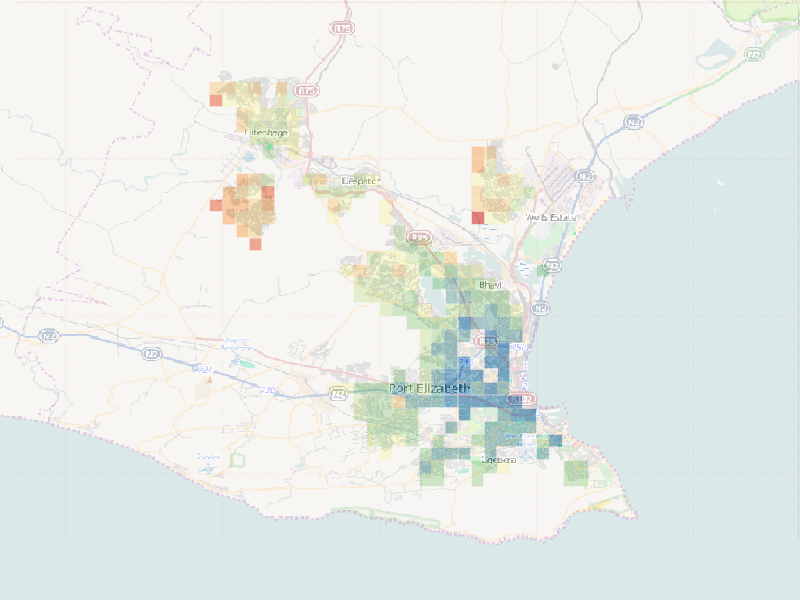
\includegraphics[width=0.99\hsize,trim=2cm 2.5cm 2cm 3cm,clip]{extending/figures/accessibility/w_freeSpeed_snapshot.png}}%
{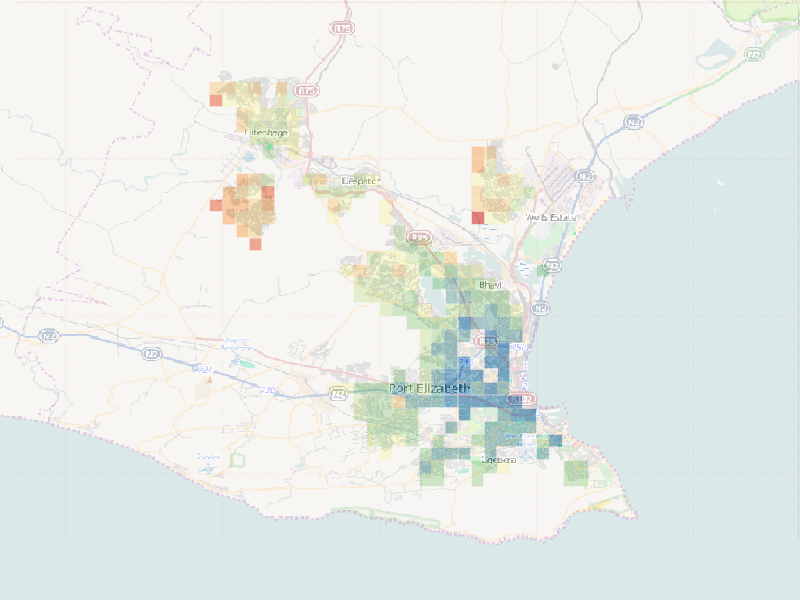
\includegraphics[width=0.99\hsize]{extending/figures/accessibility/w_freeSpeed_snapshot.png}}%
{}

%To use this functionality a \lstinline{GridBasedAccessibilityControllerListenerV3} needs to be added to the controller.
%Alternatively, if the calculation based on some given zonation system is desidered, the 
%\lstinline{ZoneBasedAccessibilityControllerListenerV3} can be used.
%
%BuettnerEtAl2010Erreichbarkeitsatlas, p.49
%Das Raumstrukturmodell stellt im Kern eine Einteilung des Unterschungsgebiets der EMM in kleine Zellen dar. Fur den 
%Erreichbarkeitsatlas wurden zu diesem Zweck die Gemeinden herangezogen, welche auf der Betrachtungsebene der gesamten 
%EMM eine ausreichende raumliche Genauigkeit bieten. Die Gemeinden sind zudem die kleinste raumliche Einheit, fur die
%von Seiten des Statistischen Landesamtes Bayern die benötigten Strukturdaten (z.B. Einwohner- und Beschaftigtenzahlen)
%kostenfrei und einheitlicher Form zur Verfügung gestellt werden.
%
%BuettnerEtAl2010Erreichbarkeitsatlas, p.50
%Erreichbarkeitsmodelle verwenden in der Regel Zellensysteme um raumliche Strukturdaten abzubilden. Der wesentliche Grund
%hierfur ist die große Zahl der einzelnen Datenelemente (z.B. Einwohner, Arbeitsplätze etc.). Wenngleich sich 
%Erreichbarkeitsindikatoren theoretisch auch vollständig disaggregiert berechnen ließen, scheitert dies in der 
%Praxis doch am Rechenaufwand aber auch an der Verfugbarkeit entsprechend feinteiliger Daten. Gangige Praxis ist es 
%deswegen, dass Untersuchungsgebiet in Zellen einzuteilen und die Raumstrukturdaten entsprechend dieser Zellstruktur 
%zusammenzufassen

\mnote{calculation procedure}
The concrete calculation of the accessibility $A_i$ of a given origin location $i$ to opportunity locations $k$ 
works as follows: The origin location $i$ and opportunity locations $k$ are assigned to a congested road network 
with time-dependent travel times as it is simulated in \gls{matsim}. For every $i$ a so-called 
\textit{least cost path tree} computation runs through the network and determines the best route, and thus the 
least negative travel utility $V_{ik}$, to each opportunity location $k$ by using Dijkstra's shortest path 
algorithm \citep{Dijkstra1959ShortestPath}. The best route from $i$ to $k$ depends on the given generalized cost 
such as link travel times or distances. Dependent on the setting in the config chosen by the user, 
these link travel times may either be free-flow travel 
times or travel times on the ``congested'' transport network (see section \ref{sec:integrated}). The least cost 
path tree computation, anchored at the origin $i$, starts at a specific time-of-day, and then executes a 
time-dependent Dijkstra shortest path algorithm \citep{LefebvreBalmer2007Fastshortestpath}. Accessibility of the 
same location at a different time-of-day will usually be different, since congestion patterns are different.
Once the least cost path tree has explored all nodes, the resulting disutilities $V_{ik}$ for all opportunities 
are queried and the accessibility is calculated as stated in Equation~(\ref{eq:accessibility:logsum0}).
%
A crucial question is how to choose the point, \ie the coordinate, where the accessibility computation is anchored. 
Most quantitative accessibility tools use geographical centroids of given zones. This is also true in case the 
zone-based \gls{matsim} accessibility computation is selected. Alternative ways to select a centroid (\eg 
land-use-based centroids \citep{BuettnerEtAl2010Erreichbarkeitsatlas}) are discussed as well. In case the 
grid-based (cell-based) \gls{matsim} accessibility computation is selected, the question of which point to
select as representative for a spatial zone centroids becomes less irrelevant as cell are usually not
selected to be as large.

%BuettnerEtAl2010Erreichbarkeitsatlas, p.55
%Die Anbindung der Regionalzellen an das OpenStreet-Netzwerk erfolgt zunächst am geometrischen Mittelpunkt einer Zelle. 
%Von diesem aus wird das nachstgelegene Netzelement ermittelt und angebunden. Perspektivisch konnte statt dem geometrischen 
%Mittelpunkt auch – unter Verwendung von Flächennutzungsdaten (vgl. Kapitel 3.5.1.2) – der Nutzungsschwerpunkt ermittelt 
%und die Zelle daruber angebunden werden.

%the following is rather directly adapted from NicolaiNagel2012HiResAccessibilityMethodInBook
Especially, if the granularity of the grid-based \gls{matsim} accessibility computation is increased, the fact that 
origin and opportunity locations do not necessarily lie on the network becomes more and more relevant. To keep the 
approach consistent, the calculation of $V_{ik}$, thus, has to include the disutility of travel to overcome the gap 
between locations and the road network. Therefore, the disutility of travel calculated by running the ``least cost 
path tree'' computation on the network has to be supplemented by the disutility to access the network from the origin 
(network access) and the disutility to access the destination from network (network egress). For origin locations $i$, 
the shortest distance to the network is either given by (i) the Euclidean distance to the nearest node or (ii) the 
orthogonal distance to the nearest link on the network.
%If the mapping of location $i$ is to a link, as in case (ii), $V_{ik}$ further includes the travel disutility to 
%overcome the distance to the nearest node. The travel costs on the link are calculated by dividing the distance to 
%the node by the travel speed of the considered transport mode, e.g.\ car (free speed or congested car travel times 
%at a given time-of-day), bicycle, or walk.
For opportunity ($=$ destination) locations $k$, the Euclidean distance to the nearest node is used to determine
the shortest distance to the network.

%In all cases, the generalized cost of travel is computed according to the same principles as it is done in the dynamic 
%traffic assignment; in the current implementation, also the utility weights are the same.  
%
%One consequence of this is that the accessibility in fact refers to a certain time-of-day.  Technically, the least 
%cost path tree computation, anchored at the origin $i$, starts at a specific time-of-day, and then executes a 
%time-dependent Dijkstra shortest path algorithm \citep{LefebvreBalmer2007Fastshortestpath}.  Accessibility of the 
%same location at a different time-of-day will usually be different, since congestion patterns are different.

%When looking at high-resolution accessibility calculations, there are, in fact,
%two resolutions to consider: One that defines for how many origins $i$ the
%accessibility is to be computed. And a second one that defines to what level
%the opportunities $k$ are to be resolved.

%\paragraph{Spatial resolution of the origin} In the present implementation, the origin side can be calculated for
%two spatial units, cells or zones. Their spatial resolution determines the
%number of measuring points for which the accessibility will be computed:
%\begin{itemize}
%	\item \textbf{Cell-based Approach}: In this approach the study area is
%	subdivided into square cells, where the resulting cell centroids
%	serve as origins or measuring points for the accessibility calculation; see
%	Fig.~\ref{fig:cellcentroids}. The spatial resolution depends on the
%	selected cell size, which is configurable.
%	\item \textbf{Zone-based Approach}: This approach uses zone
%	centroids as measuring points, see Fig.~\ref{fig:zonecentroids}. The
%	centroid coordinates can be obtained from a variety of definitions. In
%	this paper, they are determined by averaging all parcel coordinates that
%	belong to a zone. This corresponds to weighting each parcel equally; this
%	may not be justified when, say, the number of residents or households
%	varies strongly between parcels. 
%	The number of measuring points is defined by the number of
%	zones.
%\end{itemize}
%%
%In both cases, the accessibility computation is valid for the measuring point.
%
%In the grid-based approach it is then assumed that accessibility for in-between locations should be interpolated.
%
%In contrast, for the zone-based approach the accessibility of the measuring point is taken as 
%representative for the whole zone.  In consequence, the choice of the procedure of how to generate 
%the measuring point for the zone-based approach has an influence on the results.  There is no 
%corresponding choice for the grid-based approach, removing one element of arbitrariness compared 
%to the zone-based approach.

%The following paragraphs concentrate on the cell-based approach.
%Nevertheless, the
%calculation procedure of the logsum term is the same for both approaches.
%
%Opportunity locations such as work places are given by land-use. As stated earlier, they are attached to the
%nearest network node. 

The assumption that opportunity locations are attached to the nearest network \textit{node} rather than the nearest 
network \textit{element} is, in fact, the only approximation that the \gls{matsim}
accessibility extension makes with respect to the spatial resolution of opportunities 
\citep{NicolaiNagel2012HiResAccessibilityMethodInBook}. This assumption is unlikely to alter accessibility 
results significantly, but offers a great potential for the
optimization of computational performance, which has often been a major obstacle to higher-resolved 
accessibility computations \citep{Kwan1998PointBasedAccessibility, BuettnerEtAl2010Erreichbarkeitsatlas}. 
In the concrete case of the \gls{matsim} accessibility computation, the exploration of the entire network 
by the ``least cost path tree'' is a computationally expensive task.

Thanks to the aforementioned assumption that opportunity locations are attached to the nearest network 
\textit{node}, it is sufficient to sum over all opportunities $k$ attached to a node $j$ only 
once. The travel disutility $V_{ik}$ can be decomposed as
\begin{equation}
V_{ik} = V_{ij} + V_{jk} \ \forall k \in j \ ,
\end{equation}
where $k \in j$ refers to all opportunities $k$ attached to node $j$. With
\begin{equation}
\sum_{k \in j} e^{ V_{ik}} 
%
= \sum_{k \in j} e^{ (V_{ij}+ V_{jk})} 
%
= \sum_{k \in j} e^{ V_{ij}} e^{ V_{jk}} 
%
= e^{ V_{ij}} \sum_{k \in j} e^{ V_{jk}} 
%
=: e^{ V_{ij}} \cdot Opp_j
\end{equation} 
it is sufficient to compute $Opp_j$ once for every network node $j$, and compute accessibilities as
\begin{equation}
A_i = ln \sum_k e^{ V_{ik}}
%
= ln \sum_j e^{ V_{ij}} \cdot Opp_j \ .
\end{equation}

Therefore, the loop that performs the calculation does not have to run over all opportunities $k$, but instead just 
over (the usually significantly lower number) of network nodes $j$.

Similarly, for each origin location $i$, the nearest node on the road network is identified so that locations that 
share the same node have the same travel disutilities on the network. Just as in the case for destinations, the 
least cost path tree is, therefore, executed only once and the calculated disutilities on the network are reused 
for all $i$ that are mapped on the same node. Just the calculation of the travel disutility of network access needs
to be done individually for each origin $i$. \citet{NicolaiNagel2012HiResAccessibilityMethodInBook} show that due 
to this runtime optimization, computation time increases sub-linearly with resolution. At the same time, they find 
that no significant further insights can be gained by increasing the resolution beyond 100\,meters.

The application example \lstinline{RunAccessibilityExample} (see \url{http://matsim.org/javadoc} $\to$ 
accessibility $\to$ \lstinline{RunAccessibilityExample}) performs multiple accessibility computation for different
types of activity facilities (\ie accessibility of workplaces or accessibility
of leisure facilities) by adding multiple instances of \lstinline{GridBasedAccessibilityControlerListenerV3}
to the \gls{matsim} controller. Other ways of performing distinct accessibility assessments for parts of
the land-use system are equally possible. Figure \ref{fig:accessibility-nmbm} is an example for accessibilities
of work places.

\section{Conclusion}
There are many different approaches to calculate accessibilities. As has been pointed out, most approaches focus
on a particular component of accessibility, while other components that influence accessibility are 
represented only in a limited way. Accessibility computations used in transport planning, for instance, represent 
transport networks, and thus the transport component of accessibility very well, while they mostly do not represent
properties of facilities or temporal effects. As pointed out by \citet{Geurs2004AccessibilityReview}, however, it
would be desirable if an accessibility computation considered all components of accessibility (\ie the transport, 
the land-use, the temporal, and the individual component) well. The accessibility extension of \gls{matsim} can 
be seen as an approach to achieve this. 

First, the dynamics of the transport system are represented by the integration of the accessibility 
computation with \gls{matsim} dynamic traffic simulation. 
Second, land use is represented in a very disaggregate way as locations and attributes of single facilities are
taken into account.
Third, the temporal dimension can be observed by respecting opening times of facilities and time-dependent
travel times on the network, which are given as output of the \gls{matsim} dynamic traffic simulation.
%As \gls{matsim} is a simulation that runs second by second, the temporal dimension is represented in a very detailed way.
Finally, there is potential to take individual characteristics into account because in the \gls{matsim} simulation 
each individual is represented by its own software object, \ie an agent, whose properties could be
considered in the calculation of accessibilities.

Actual accessibility values calculated by the \gls{matsim} accessibility extension are of the form of 
\textit{potential accessibility measure} as originally defined by \citet{Hansen1959HowAccessibilityShapesLandUse}.
Owing to the specific selection of the mathematical form of the measure, results can be interpreted as 
\gls{logsum} values, which makes them suitable to be used for economic evaluations like benefit-cost analyses.
The fact that the \gls{matsim} accessibility extension can rely solely on publicly and freely available 
data, \eg data from \gls{osm}, makes it portable between different locations. By distinguishing activity facilities 
along various potential dimensions many different kinds of analyses can be conducted. In the code example given
(see \url{http://matsim.org/javadoc} $\to$ accessibility $\to$ \lstinline{RunAccessibilityExample}), for instance,
accessibilities for different kinds of land use, \ie different types of acitivy opportunities, are calculted.
Being grid- instead of zone-based (which most other accessibility tools are) certain problems associated with 
zones can be avoided. At the same time, it has been shown that computations are still computationally well
feasible, which is partly due to a runtime optimization that reuses computational steps for opportunities that 
share the same nearest network node.


%aus einer Praesentation
%Aufgabe des Staates: Grundversorgung der Bevölkerung
%Nötig: (Infrastruktur-)Maßnahmen bewerten
%Heute i.d.R. ausschließlich auf Basis verkehrs- und mobilitätsbezogener Maße
%Qualität der erreichbaren Angebote
%Nicht bewertet
%Mittels Durchschnittswerten bewertet
%Keine Aussage bzgl. etwaiger räumlicher und/oder sozialer Ungleichverteilungen
%Verteilungsmaße (z.B. generalisierter Gini-Koeffizient)
%Verortung unterversorgter Personen?
%Beitrag zur Verbesserung des Zugangs zum jeweiligen Angebot?


%public GridBasedAccessibilityControlerListenerV3(ActivityFacilities opportunities, Config config, Network network)

%do we still need the following part...????? it is already stated in the text above

%\section{Invocation}
%
%\subsection{Invocation as \enquote{Script in Java}}
%
%See \url{http://matsim.org/javadoc} $\to$ accessibility $\to$ \lstinline{RunAccessibilityExample} class for an example.



% ##################################################################################################################

% Local Variables:
% mode: latex
% mode: reftex
% mode: visual-line
% TeX-master: "../../main"
% comment-padding: 1
% fill-column: 9999
% End: 
